\chapter{Multiple regression and ANOVA}
\label{multipleRegressionAndANOVA}

The principles of simple linear regression with one numerical predictor and one numerical response lay the foundation for more sophisticated regression methods used in a wide range of challenging settings. In Chapter~\ref{multipleRegressionAndANOVA}, we explore multiple regression, which introduces the possibility of more than one predictor. We will also consider methods for analysis of variance (ANOVA), a tool useful both in practice and when learning about the mechanics of regression.

\section{Introduction to multiple regression}

Multiple regression extends the simple bivariate regression (two variables: $x$ and $y$) to the case that still has one response but may have many predictors (denoted $x_1$, $x_2$, $x_3$, ...). The method is motivated by scenarios where many variables may be simultaneously connected to an output.

We will consider Ebay auctions of a video game called \emph{Mario Kart} for the Nintendo Wii. 
The outcome variable of interest is the total price of an auction - the highest bid plus the shipping cost. But how is the total price related to characteristics of an auction? For instance, are longer auctions associated with a higher or lower prices? And, on average, how much more do buyers tend to pay for additional Wii wheels (plastic steering wheels that attach to the Wii controller) in auctions? Multiple regression will help us answer these and other questions.

The data set \data{marioKart} includes results from 143 auctions\footnote{Diez DM, Barr CD, and \c{C}etinkaya M. 2011. \emph{openintro}: OpenIntro data sets and supplemental functions. R package Version 1.2.}. Four observations from this data set are shown in Table~\ref{marioKartDataMatrix}, and descriptions for each variable are shown in Table~\ref{marioKartVariables}.
\begin{table}[ht]
\centering
\begin{tabular}{rrrrlr}
  \hline
 & totalPr & condNew & stockPhoto & duration & wheels \\ 
  \hline
1 & 51.55 &   1 & 1 & 3 &   1 \\ 
  2 & 37.04 &  0 &  1 & 7 &   1 \\ 
$\vdots$ &$\vdots$ &$\vdots$ &$\vdots$ &$\vdots$ &$\vdots$ \\
  142 & 38.76 &  0 &  0 & 7 &   0 \\ 
  143 & 54.51 &  1 &  1 & 1 &   2 \\ 
   \hline
\end{tabular}
\caption{Four observations from the \data{marioKart} data set.}
\label{marioKartDataMatrix}
\end{table}

\begin{table}
\centering\small
\begin{tabular}{lp{9.5cm}}
\hline
{\bf variable} & {\bf description} \\
\hline
\var{totalPr} & the total of the final auction price and the shipping cost, in US dollars \\
\var{condNew} & a coded two-level categorical variable, which takes value \resp{1} when the game is new and \resp{0} if the game is used \\
\var{stockPhoto} & a coded two-level categorical variable, which takes value \resp{1} if the primary photo used in the auction was a stock photo and \resp{0} if the photo was unique to that auction \\
\var{duration} & the length of the auction, in days \\
\var{wheels} & the number of Wii wheels included with the auction (a \emph{Wii wheel} is a plastic racing wheel that holds the Wii controller and is an optional but helpful accessory for playing Mario Kart Wii) \\
\hline
\end{tabular}
\caption{Variables and their descriptions for the \data{marioKart} data set.\vspace{-3mm}}
\label{marioKartVariables}
\end{table}

\subsection{Using categorical variables with two levels as predictors}

There are two predictor variables in the \data{marioKart} data set that are inherently categorical: a variable describing the condition of the game and the variable describing whether a stock photo was used for the auction. Two-level categorical variables are often coded using \resp{0}'s and \resp{1}'s, which allows them to be incorporated into a regression model in the same way as a numerical predictor:
\begin{align*}
\widehat{\var{totalPr}} = \beta_0 + \beta_1*\var{condNew}
\end{align*}
If we fit this model for total price and game condition using simple linear regression, we obtain the following regression line estimate:
\begin{align} \label{simpleLinearModelForTotalPrAndCondNew}
\widehat{\var{totalPr}} = 42.87 + 10.90*\var{condNew}
\end{align}
The \resp{0}-\resp{1} coding of the two-level categorical variable allows for a simple interpretation of the coefficient of \var{condNew}. When the game is in \resp{used} condition, the \var{condNew} variable takes a value of zero, and the total auction price predicted from the model would be $\$42.87 + \$10.90*(0) = \$42.87$. If the game is in \resp{new} condition, then the \var{condNew} variable takes value one and the total price is predicted to be $\$42.87 + \$10.90*(1) = \$53.77$. We now see clearly that the coefficient of \var{condNew} estimates the difference (\$10.90) in the total auction price when the game is new (\$53.77) versus used (\$42.87).

\begin{tipBox}{\tipBoxTitle{The coefficient of a two-level categorical variable}
The coefficient of a binary variable corresponds to the estimated difference in the outcome between the two levels of the variable.}
\end{tipBox}\vspace{-3mm}

\begin{exercise} \label{exerciseForBinaryPredictorModelForTotalPrAndStockPhoto}
The best fitting linear model for the outcome \var{totalPr} and predictor \var{stockPhoto} is
\begin{align} \label{simpleLinearModelForTotalPrAndStockPhoto}
\widehat{\var{totalPr}} = 44.33 + 4.17*\var{stockPhoto}
\end{align}
where the variable \var{stockPhoto} takes value \resp{1} when a stock photo is being used and \resp{0} when the photo is unique to that auction. Interpret the coefficient of \var{stockPhoto}.
\end{exercise}

\begin{example}{In Exercise~\ref{exerciseForBinaryPredictorModelForTotalPrAndStockPhoto}, you found that auctions whose primary photo was a stock photo tended to sell for about \$4.17 more than auctions that feature a unique photo. Suppose a seller learns this and decides to change her Mario Kart Wii auction to have its primary photo be a stock photo. Will modifying her auction in this way earn her, on average, an additional \$4.17?}
No, we cannot infer a causal relationship. It might be that there are inherent differences in auctions that use stock photos and those that do not. For instance, if we sorted through the data, we would actually notice that many of the auctions with stock photos tended to also include more Wii wheels. In this case, Wii wheels is a potential lurking variable.
\end{example}

\subsection{Including and assessing many variables in a model}

Sometimes there is underlying structure or relationship between the predictor variables. For instance, new games sold on Ebay tend to come with more Wii wheels, which may have led to higher prices for those auctions. We would like to fit a model that included all potentially important variables simultaneously, which would help us evaluate the relationship between a predictor variable and the outcome while controlling for the potential influence of other variables. This is the strategy used in \term{multiple regression}. While we remain cautious about making any causal interpretations using multiple regression, such models are a common first step in providing evidence of a causal connection.

Earlier we had constructed a simple linear model using \var{condNew} as a predictor and \var{totalPr} as the outcome. We also constructed a separate model using only \var{stockPhoto} as a predictor. Next, we want a model that uses both of these variables simultaneously and, while we're at it, we'll include the \var{duration} and \var{wheels} variables described Table~\ref{marioKartVariables}:
\begin{align}
\widehat{\var{totalPr}} &= \beta_0 + \beta_1*\var{condNew} + \beta_2*\var{stockPhoto} \notag \\
				&\qquad\  + \beta_3 * \var{duration} + \beta_4 * \var{wheels} \notag \\
\hat{y} &= \beta_0 + \beta_1 x_1 + \beta_2 x_2 + \beta_3 x_3 + \beta_4 x_4
\label{eqForMultipleRegrOfTotalPrForAllPredictors}
\end{align}
where $y$ represents the total price, $x_1$ is the game's condition, $x_2$ is whether a stock photo was used, $x_3$ is the duration of the auction, and $x_4$ is the number of Wii wheels included with the game. Just as with the single predictor case, this model may be missing important components or it might not properly represent the relationship between the total price and the available explanatory variables. However, while no model is perfect, we wish to explore the possibility that this one may fit the data reasonably well.

We estimate the parameters $\beta_0$, $\beta_1$, ..., $\beta_4$ in the same way as we did in the case of a single predictor. We select $b_0$, $b_1$, ..., $b_4$ that minimize the sum of the squared residuals:
\begin{align}\label{sumOfSqResInMultRegr}
SSE = \sum_{i=1}^{n} e_i^2
	 = \sum_{i=1}^{n} \left(y_i - \hat{y}_i\right)^2
\end{align}
We typically use a computer to minimize this sum and compute point estimates, as shown in the sample output in Table~\ref{outputForMultipleRegrOutputForAllPredictors}. Using this output, we identify the point estimates $b_i$ of each $\beta_i$, just as we did in the one-predictor case.

\begin{table}[ht]
\centering
\begin{tabular}{rrrrr}
  \hline
 & Estimate & Std. Error & t value & Pr($>$$|$t$|$) \\ 
  \hline
(Intercept) & 36.2110 & 1.5140 & 23.92 & 0.0000 \\ 
  condNew & 5.1306 & 1.0511 & 4.88 & 0.0000 \\ 
  stockPhoto & 1.0803 & 1.0568 & 1.02 & 0.3085 \\ 
  duration & -0.0268 & 0.1904 & -0.14 & 0.8882 \\ 
  wheels & 7.2852 & 0.5547 & 13.13 & 0.0000 \\ 
   \hline
   &&&\multicolumn{2}{r}{$df=136$}
\end{tabular}
\caption{Output for the regression model where \var{totalPr} is the outcome and \var{condNew}, \var{stockPhoto}, \var{duration}, and \var{wheels} are the predictors.}
\label{outputForMultipleRegrOutputForAllPredictors}
\end{table}

\begin{termBox}{\tBoxTitle{Multiple regression model}
A multiple regression model is a linear model with many predictors. In general, we write the model as
\begin{align*}
\hat{y} = \beta_0 + \beta_1 x_1 + \beta_2 x_2 + \cdots + \beta_p x_p
\end{align*}
when there are $p$ predictors. We often estimate the $\beta_i$ parameters using a computer.}%, which minimizes the sum of the squared residuals, shown in Equation~\eqref{sumOfSqResInMultRegr}.}
\end{termBox}

\begin{exercise} \label{eqForMultipleRegrOfTotalPrForAllPredictorsWithCoefficients}
Write out the model in Equation~\eqref{eqForMultipleRegrOfTotalPrForAllPredictors} using the point estimates from Table~\ref{outputForMultipleRegrOutputForAllPredictors}. How many predictors are there in this model? Answers in the footnote\footnote{$\hat{y} = 36.21 + 5.13x_1 + 1.08x_2 - 0.03x_3 + 7.29x_4$, and there are $p=4$ predictor variables.}.
\end{exercise}

\begin{exercise}
What does $\beta_4$, the coefficient of variable $x_4$ (Wii wheels), represent? What is the point estimate of $\beta_4$? Answers in the footnote\footnote{It is the average difference in auction price for each additional Wii wheel included when holding the other variables constant. The point estimate is $b_4 = 7.29$.}.
\end{exercise}

\begin{exercise} \label{computeMultipleRegressionResidualForMarioKart}
Compute the residual of the first observation in Table~\ref{marioKartDataMatrix} on page~\pageref{marioKartDataMatrix}. Hint: use the equation from Exercise~\ref{eqForMultipleRegrOfTotalPrForAllPredictorsWithCoefficients}. Answer in the footnote\footnote{$e_i = y_i - \hat{y_i} = 51.55 - 49.62 = 1.93$, where 49.62 was computed using the predictor values for the observation and the equation identified in Exercise~\ref{eqForMultipleRegrOfTotalPrForAllPredictorsWithCoefficients}.}.
\end{exercise}

\begin{example}{The coefficients for $x_1$ (\var{condNew}) and $x_2$ (\var{stockPhoto}) are different than in the two simple linear models shown in Equations~\eqref{simpleLinearModelForTotalPrAndCondNew} and~\eqref{simpleLinearModelForTotalPrAndStockPhoto}. Why might there be a difference?} \label{colinearityOfCondNewAndStockPhoto}
If we examined the data carefully, we would see that some predictors are correlated. For instance, when we estimated the connection of the outcome \var{totalPr} and predictor \var{stockPhoto} using simple linear regression, we were unable to control for other variables like \var{condNew}. That model was biased by the lurking variable \var{condNew}. When we use both variables, this particular underlying and unintentional bias is reduced or eliminated (though bias from other lurking variables may still remain).
\end{example}

Example~\ref{colinearityOfCondNewAndStockPhoto} describes a common issue in multiple regression: correlation among predictor variables. We say the two predictor variables are \term{collinear} when they are correlated, and this collinearity complicates model estimation. While it is impossible to prevent collinearity from arising in observational data, experiments are usually designed to prevent predictors from being correlated.

\subsection{Adjusted $R^2$ as a better estimate of explained variance}

We first used $R^2$ in Section~\ref{fittingALineByLSR} to determine the amount of variability in the response that was explained by the model:
\begin{align*}
R^2 = 1 - \frac{\text{variability in residuals}}{\text{variability in the outcome}}
	= 1 - \frac{Var(e_i)}{Var(y_i)}
\end{align*}
where $e_i$ represents the residuals of the model and $y_i$ the outcomes. This equation remains valid in the multiple regression framework, but a small enhancement can often be even more informative.

\begin{exercise} \label{computeUnadjustedR2ForAllPredictorsInMarioKart}
The variance of the residuals for the model given in Exercise~\ref{computeMultipleRegressionResidualForMarioKart} is 23.34, and the variance of the total price in all the auctions is 83.06. Verify the $R^2$ for this model is 0.719.
\end{exercise}

This strategy for estimating $R^2$ is okay when there is just a single variable. However, it becomes less helpful when there are many variables. The regular $R^2$ is actually a biased estimate of the amount of variability explained by the model. To get a better estimate, we use the adjusted $R^2$.

\begin{termBox}{\tBoxTitle{Adjusted $\mathbf{R^2}$ as a tool for model assessment}
The \termsub{adjusted $\mathbf{R^2}$}{adjusted $R^2$} is computed as
\begin{align*}
R_{adj}^{2} = 1-\frac{Var(e_i) / (n-p-1)}{Var(y_i) / (n-1)}
	= 1-\frac{Var(e_i)}{Var(y_i)} \times \frac{n-1}{n-p-1}
\end{align*}
where $n$ is the number of cases used to fit the model and $p$ is the number of predictor variables in the model.}
\end{termBox}

Because $p$ is never negative, the adjusted $R^2$ will be smaller -- often times just a little smaller -- than the unadjusted $R^2$. The reasoning behind the adjusted $R^2$ lies with the \term{degrees of freedom} associated with each variance\footnote{In multiple regression, the degrees of freedom associated with the variance of the estimate of the residuals is $n-p-1$, not $n-1$. For instance, if we were to make predictions for new data using our current model, we would find that the unadjusted $R^2$ is an overly optimistic estimate of the reduction in variance in the response, and using the degrees of freedom in the adjusted $R^2$ formula helps correct this bias.}.

\begin{exercise}
There were $n=141$ auctions in the \data{marioKart} data set and $p=4$ predictor variables in the model. Use $n$, $p$, and the variances from Exercise~\ref{computeUnadjustedR2ForAllPredictorsInMarioKart} to verify $R_{adj}^2 = 0.711$ for the Mario Kart model.
\end{exercise}

\begin{exercise}
Suppose you added another predictor to the model, but the variance of the errors $Var(e_i)$ didn't go down. What would happen to the $R^2$? What would happen to the adjusted $R^2$? Answers in the footnote\footnote{The unadjusted $R^2$ would stay the same and the adjusted $R^2$ would go down.}.
\end{exercise}

The idea that a predictor that doesn't explain any extra variance would actually ``hurt'' the adjusted $R^2$ highlights a common sentiment in statistics: avoid making a model more complicated than it needs to be.

%%%%%
\section{Model selection}
\label{modelSelection}

The best model is not always the most complicated. Sometimes including variables that are not evidently important can actually reduce the accuracy of predictions. In this section we discuss model selection strategies, which will help us eliminate variables that are less important from the model.

In this section, and in practice, the model that includes all available explanatory variables is often referred to as the \term{full model}. Our goal is assess whether the full model is the best model. If it isn't, we want to identify a smaller model that is preferable.

\subsection{Identifying variables that may not be helpful in the model}

Table~\ref{outputForMultipleRegrOutputForAllPredictors2} provides a summary of the regression output for the full model. The last column of the table lists p-values that can be used to assess hypotheses of the following form:
\begin{itemize}
\setlength{\itemsep}{0mm}
\item[$H_0$:] $\beta_i = 0$ when the other explanatory variables are included in the model.
\item[$H_A$:] $\beta_i \neq 0$ when the other explanatory variables are included in the model.
\end{itemize}
\begin{table}[ht]
\centering
\begin{tabular}{rrrrr}
  \hline
 & Estimate & Std. Error & t value & Pr($>$$|$t$|$) \\ 
  \hline
(Intercept) & 36.2110 & 1.5140 & 23.92 & 0.0000 \\ 
  condNew & 5.1306 & 1.0511 & 4.88 & 0.0000 \\ 
  stockPhoto & 1.0803 & 1.0568 & 1.02 & 0.3085 \\ 
  duration & -0.0268 & 0.1904 & -0.14 & 0.8882 \\ 
  wheels & 7.2852 & 0.5547 & 13.13 & 0.0000 \\ 
   \hline
   &&&\multicolumn{2}{r}{$df=136$}
\end{tabular}
\caption{The fit for the full regression model. This table is identical to Table~\ref{outputForMultipleRegrOutputForAllPredictors}.}
\label{outputForMultipleRegrOutputForAllPredictors2}
\end{table}

\begin{example}{The coefficient of \var{condNew} has a $t$ test statistic of $T=4.88$ and a p-value for its corresponding hypotheses ($H_0: \beta_1 = 0$, $H_A: \beta_1 \neq 0$) of about zero. How can this be interpretted?}
If we keep all the other variables in the model and add no others, then there is strong evidence that a game's condition (new or used) has a real relationship with the total auction price.
\end{example}

\begin{example}{Is there strong evidence that using a stock photo is related to the total auction price?}
The $t$ test statistic for \var{stockPhoto} is $T=1.02$ and the p-value is about 0.31. There is not strong evidence that using a stock photo in an auction is related to the total price of the auction. We might consider removing the \var{stockPhoto} variable from the model.
\end{example}

\begin{exercise}
Identify the p-values for both the \var{duration} and \var{wheels} variables in the model. Is there strong evidence supporting the connection of these variables with the total price in the model?
\end{exercise}

There is not statistically significant evidence that either \var{stockPhoto} or \var{duration} are meaningfully contributing to the model. If the coefficients of these variables are not zero, their association with the outcome variable is probably weak. Next we consider common strategies for pruning such variables from a model.\vspace{-1mm} %ZZQ Formatting

\begin{tipBox}{\tipBoxTitle{Using adjusted $R^2$ instead of p-values for model selection}
The adjusted $R^2$ may be used as an alternative to p-values for model selection, where a higher adjusted $R^2$ represents a better model fit. For instance, we could compare two models using their adjusted $R^2$, and the model with the higher adjusted $R^2$ would be preferred. This approach tends to include more variables in the final model when compared to the p-value approach.}
\end{tipBox}\vspace{-4.5mm} %ZZQ Formatting

\subsection{Two model selection strategies}

Two common strategies for adding or removing variables in a multiple regression model are called \emph{backward-selection} and \emph{forward-selection}. These techniques are often referred to as \term{stepwise} model selection strategies, because they add or delete one variable at a time as they ``step'' through the candidate predictors. We will discuss these strategies in the context of the p-value approach, however, the adjusted $R^2$ approach may be employed as an alternative.

The \term{backward-elimination} strategy starts with the model that includes all potential predictor variables. One-by-one variables are eliminated from the model until only variables with statistically significant p-values remain. The strategy within each elimination step is to drop the variable with the largest p-value, refit the model, and reassess the inclusion of all variables.

\begin{example}{Results corresponding to the \emph{full model} for the {\tt marioKart} data are shown in Table~\ref{outputForMultipleRegrOutputForAllPredictors2}. How should we proceed under the backward-elimination strategy?}
There are two variables with coefficients that are not statistically different from zero: \var{stockPhoto} and \var{duration}. We first drop the \var{duration} variable since it has a larger corresponding p-value, \emph{then we refit the model}. A regression summary for the new model is shown in Table~\ref{outputForMultipleRegrOutputForAllPredictorsButDuration}.

In the new model, there is not strong evidence that the coefficient for \var{stockPhoto} is different from zero (even though the p-value dropped a little) and the other p-values remain very small. So again we eliminate the variable with the largest non-significant p-value, \var{stockPhoto}, and refit the model. The updated regression summary is shown in Table~\ref{outputForMultipleRegrOutputForAllPredictorsButDurationAndStockPhoto}.

In the latest model, we see that the two remaining predictors have statistically significant coefficients with p-values of about zero. Since there are no variables remaining that could be eliminated from the model, we stop. The final model includes only the \var{condNew} and \var{wheels} variables in predicting the total auction price:
\begin{align*}
\hat{y} \ \ = \ \ b_0 + b_1x_1 + b_4x_4 \ \ = \ \ 36.78 + 5.58x_1 + 7.23x_4
\end{align*}
As an alternative description of how we could have performed this model selection strategy using adjusted $R^2$, please see the footnote\footnote{At each elimination step, we refit the model without each of the variables up for potential elimination (e.g. in the first step, we would fit four models, where each would be missing a different predictor). If one of these smaller models has a higher adjusted $R^2$ than our current model, we pick the smaller model with the largest adjusted $R^2$. Had we used the adjusted $R^2$ criteria, we would have kept the \var{stockPhoto} variable in this backwards-elimination example.}.
\end{example}
\begin{table}[ht]
\centering
\begin{tabular}{rrrrr}
  \hline
 & Estimate & Std. Error & t value & Pr($>$$|$t$|$) \\ 
  \hline
(Intercept) & 36.0483 & 0.9745 & 36.99 & 0.0000 \\ 
  condNew & 5.1763 & 0.9961 & 5.20 & 0.0000 \\ 
  stockPhoto & 1.1177 & 1.0192 & 1.10 & 0.2747 \\ 
  wheels & 7.2984 & 0.5448 & 13.40 & 0.0000 \\ 
   \hline
  &&&&\small$df=137$
\end{tabular}
\caption{The output for the regression model where \var{totalPr} is the outcome and the duration variable has been eliminated from the model.}
\label{outputForMultipleRegrOutputForAllPredictorsButDuration}
\end{table}
\begin{table}[ht]
\centering
\begin{tabular}{rrrrr}
  \hline
 & Estimate & Std. Error & t value & Pr($>$$|$t$|$) \\ 
  \hline
(Intercept) & 36.7849 & 0.7066 & 52.06 & 0.0000 \\ 
  condNew & 5.5848 & 0.9245 & 6.04 & 0.0000 \\ 
  wheels & 7.2328 & 0.5419 & 13.35 & 0.0000 \\ 
   \hline
  &&&&\small$df=138$
\end{tabular}
\caption{The output for the regression model where \var{totalPr} is the outcome and the duration and stock photo variables have been eliminated from the model.}
\label{outputForMultipleRegrOutputForAllPredictorsButDurationAndStockPhoto}
\end{table}

Notice that the p-value for \var{stockPhoto} changed a little from the full model (0.309) to the model that did not include the \var{duration} variable (0.275). It is common for p-values of one variable to change, due to collinearity, after eliminating a different variable. This fluctuation emphasizes the importance of refitting a model after each variable elimination step. The p-values tend to change dramatically when the eliminated variable is highly correlated with another variable in the model.



The \term{forward-selection} strategy is the reverse of the backward-elimination technique. Instead of eliminating variables one-at-a-time, we add variables one-at-a-time until we cannot find any variables that present strong evidence of their importance in the model.

\begin{example}{Construct a model for the \data{marioKart} data set using the forward-selection strategy.}
We start with the model that includes no variables. Then we fit each of the possible models with just one variable. That is, we fit the model including just the \var{condNew} predictor, then the model just including the \var{stockPhoto} variable, then a model with just \var{duration}, and a model with just \var{wheels}. Each of the four models (yes, we fit four models!) provides a p-value for the coefficient of the predictor variable. Out of these four variables, the \var{wheels} variable had the smallest p-value. Since its p-value is less than 0.05 (the p-value was smaller than 2e-16), we add the Wii wheels variable to the model. Once a variable is added in forward-selection, it will be included in all models considered and in the final model.

Since we successfully found a first variable to add, we consider adding another. We fit three new models: (1) the model including just the \var{condNew} and \var{wheels} variables (output in Table~\ref{outputForMultipleRegrOutputForAllPredictorsButDurationAndStockPhoto}), (2) the model including just the \var{stockPhoto} and \var{wheels} variables, and (3) the model including only the \var{duration} and \var{wheels} variables. Of these models, the first had the lowest p-value for its new variable (the p-value corresponding to \var{condNew} was 1.4e-08). Because this p-value is below 0.05, we add the \var{condNew} variable to the model. Now the final model is guaranteed to include both the condition and Wii wheels variables.

We repeat the process a third time, fitting two new models: (1) the model including the \var{stockPhoto}, \var{condNew}, and \var{wheels} variables (output in Table~\ref{outputForMultipleRegrOutputForAllPredictorsButDuration}) and (2) the model including the \var{duration}, \var{condNew}, and \var{wheels} variables. The p-value corresponding to \var{stockPhoto} in the first model (0.275) was smaller than the p-value corresponding to \var{duration} in the second model (0.682). However, since this smaller p-value was not below 0.05, there was not strong evidence that it should be included in the model. Therefore, neither variable is added and we are finished.

The final model is the same as that arrived at using the backward-selection strategy: we include the \var{condNew} and \var{wheels} variables into the final model. See the footnote for how we would have proceded had we used the $R_{adj}^2$ criteria instead of examining p-values\footnote{Rather than look for variables with the smallest p-value, we look for the model with the largest $R_{adj}^2$. Using the forward-selection strategy, we start with the model with no predictors. Next we look at each model with a single predictor. If one of these models has a larger $R_{adj}^2$ than the model with no variables, we use this new model. We repeat this procedure, adding one variable at a time, until we cannot find a model with a smaller $R_{adj}^2$. If we had done the forward-selection strategy using $R_{adj}^2$, we would have arrived at the model including \var{condNew}, \var{stockPhoto}, and \var{wheels}, which is a slightly larger model than we arrived at using the p-value approach.}.
\end{example}

\begin{termBox}{\tBoxTitle{Model selection strategies}
The backward-elimination strategy begins with the largest model and eliminates variables one-by-one until we are satisfied that all remaining variables are important to the model. The forward-selection strategy starts with no variables included in the model, then it adds in variables according to their importance until no other important variables are found.}
\end{termBox}

There is no guarantee that the backward-elimination and forward-selection strategies will arrive at the same final model regardless of whether we are using the p-value or $R_{adj}^2$ criteria. If the backwards-elimination and forward-selection strategies are both tried and they arrive at different models, one option is to choose between the models using the $R_{adj}^2$ criteria (other options exist but are beyond the scope of this book).

%There is also no guarantee that the forward-selection strategy will result in a model where all included variables have coefficients that are statistically different from zero, regardless of whether the p-value or $R_{adj}^2$ criteria is used. For instance, the first variable added may no longer be statistically significant after adding in other variables.

It is generally acceptable to use just one strategy, usually backward-elimination, and report the final model after verifying the conditions for fitting a linear model are reasonable.

%%%%%
\section{Checking model assumptions using graphs}

Multiple regression methods using the model
\begin{align*}
\hat{y} &= \beta_0 + \beta_1x_1 + \beta_2x_2 + \cdots + \beta_px_p
\end{align*}
generally depend on the following four assumptions:
\begin{enumerate}
\setlength{\itemsep}{0mm}
\item the residuals of the model are nearly normal,
\item the variability of the residuals is nearly constant,
\item the residuals are independent, and
\item each variable is linearly related to the outcome.
\end{enumerate}
Simple and effective plots can be used to check each of these assumptions.
\begin{description}
\item[Normal probability plot.] A normal probability plot of the residuals is shown in Figure~\ref{mkDiagnosticNormalQuantilePlot}. While the plot exhibits some minor irregularities, there are no outliers that might be cause for concern. In a normal probability plot for residuals, we tend to be most worried about residuals that appear to be outliers, since these indicate long tails in the distribution of residuals.
\begin{figure}
\centering
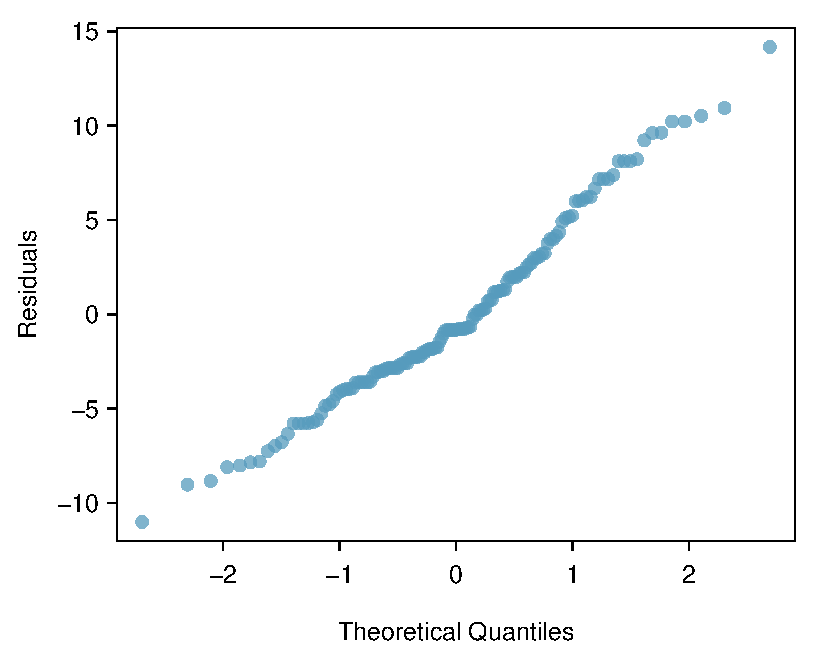
\includegraphics[width=0.71\textwidth]{08/figures/marioKartDiagnostics/mkDiagnosticNormalQuantilePlot}
\caption{A normal probability plot of the residuals is helpful in identifying observations that might be outliers.}
\label{mkDiagnosticNormalQuantilePlot}
\end{figure}
\item[Absolute values of residuals against fitted values.] A plot of the absolute value of the residuals against their corresponding fitted values ($\hat{y}_i$) is shown in Figure~\ref{mkDiagnosticEvsAbsF}. This plot is helpful to check the condition that the variance of the residuals is approximately constant. We don't see any obvious deviations from constant variance in this example.
\begin{figure}
\centering
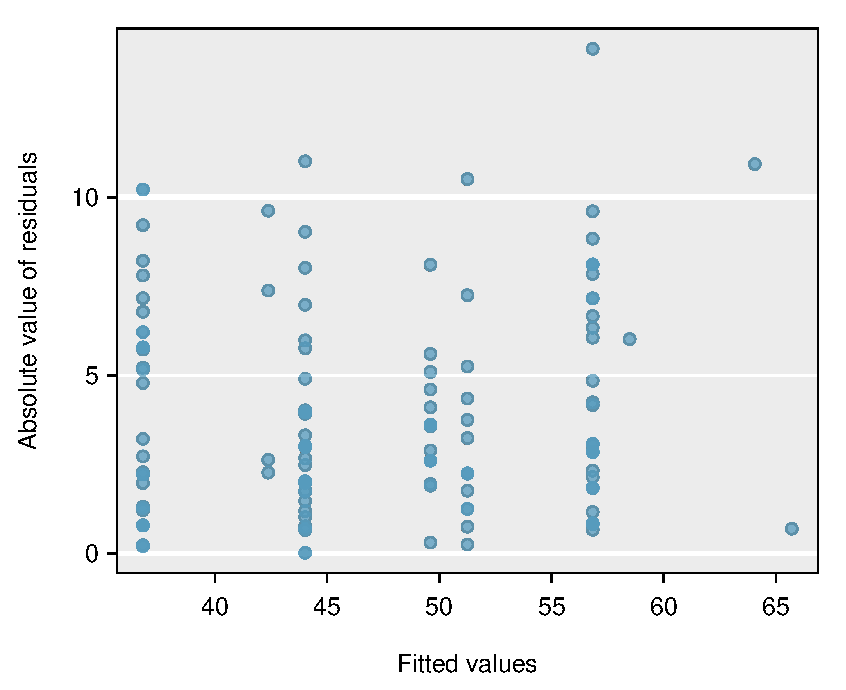
\includegraphics[width=0.72\textwidth]{08/figures/marioKartDiagnostics/mkDiagnosticEvsAbsF}
\caption{Comparing the absolute value of the residuals against the fitted values ($\hat{y}_i$) is helpful in identifying deviations from the constant variance assumption.}
\label{mkDiagnosticEvsAbsF}
\end{figure}
\item[Residuals in order of their data collection.] A plot of the residuals in the order their corresponding auctions were observed is shown in Figure~\ref{mkDiagnosticInOrder}. Such a plot is helpful in identifying any connection between cases that are close to one another, e.g. we could look for declining prices over time or if there was a time of the day when auctions tended to fetch a higher price. Here we see no structure that indicates a problem\footnote{An especially rigorous check would use \term{time series} methods. For instance, we could check whether consecutive residuals are correlated. Doing so with these residuals yields no statistically significant correlations.}.
\begin{figure}
\centering
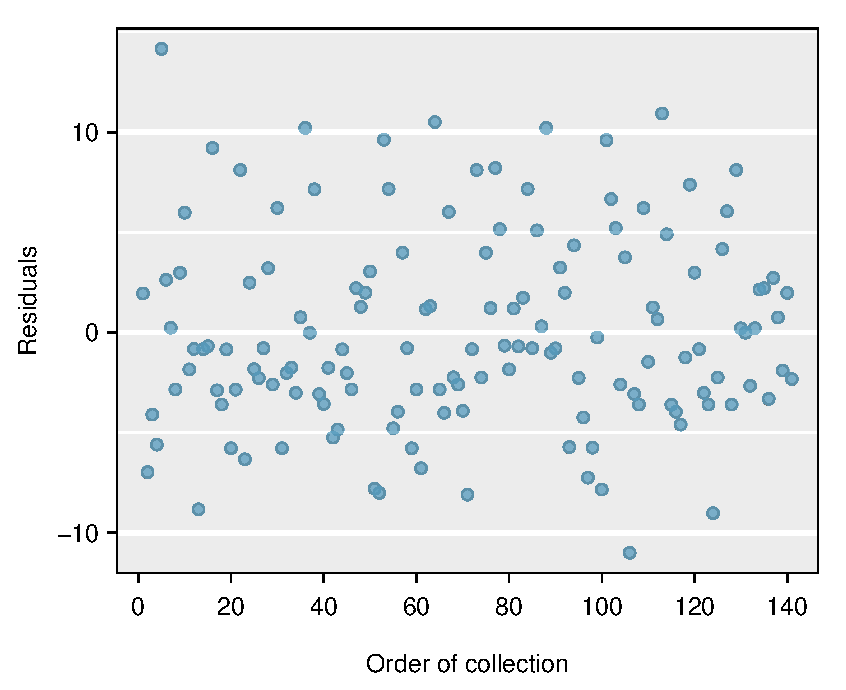
\includegraphics[width=0.72\textwidth]{08/figures/marioKartDiagnostics/mkDiagnosticInOrder}
\caption{Plotting residuals in the order that their corresponding observations were collected helps identify connections between successive observations. If it seems that consecutive observations tend to be close to each other, this indicates the independence assumption of the observations would fail.}
\label{mkDiagnosticInOrder}
\end{figure}
\item[Residuals against each predictor variable.] We consider a plot of the residuals against the \var{condNew} variable and the residuals against the \var{wheels} variable. These plots are shown in Figure~\ref{mkDiagnosticEvsVariables}. For the two-level condition variable, we are guaranteed not to see a trend, and instead we are verifying that the variability doesn't fluctuate across groups. In this example, when we consider the residuals against the \var{wheels} variable, we see structure. There appears to be curvature in the residuals, indicating the relationship is probably not linear.
\begin{figure}
\centering
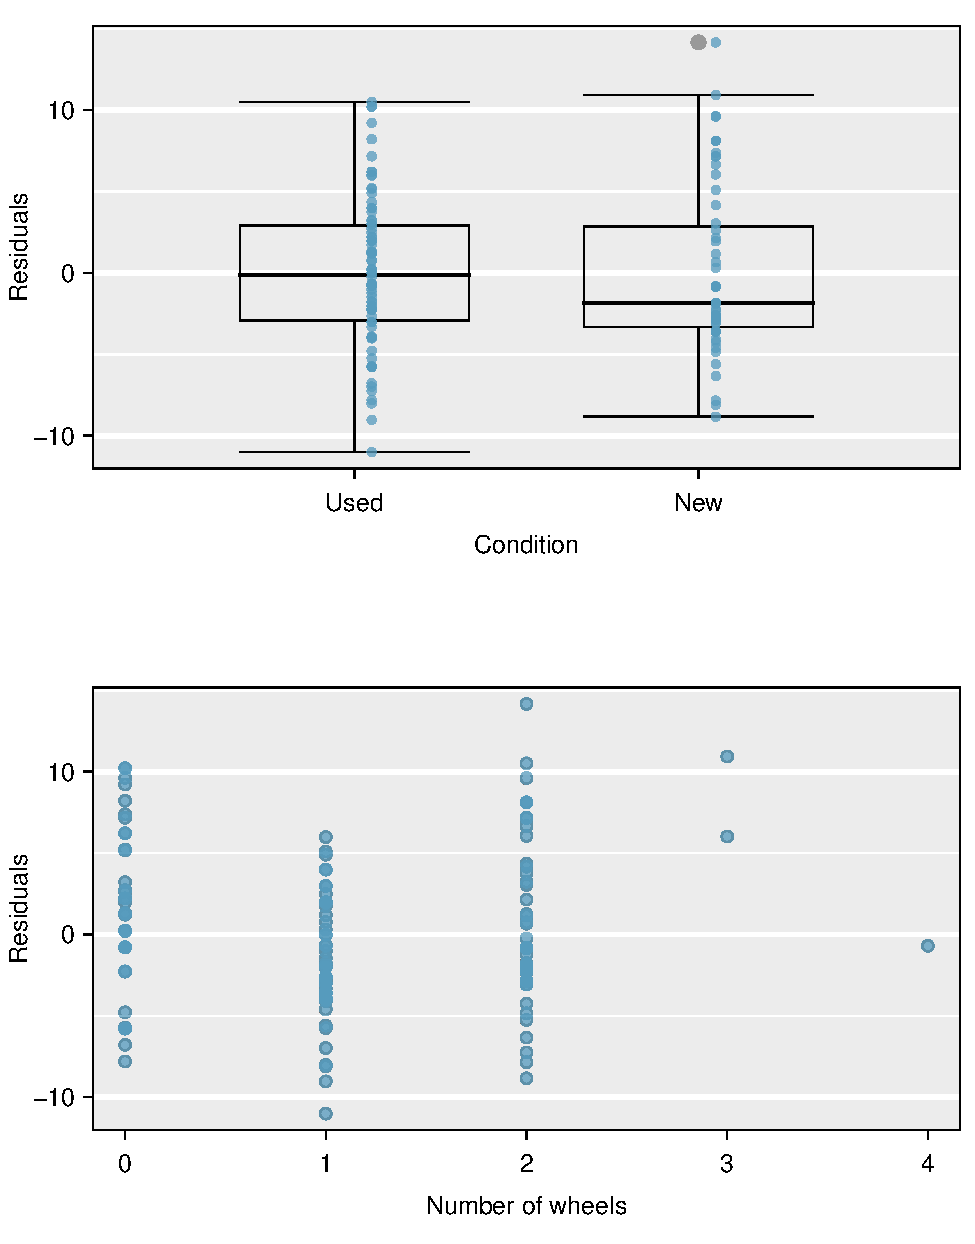
\includegraphics[width=0.85\textwidth]{08/figures/marioKartDiagnostics/mkDiagnosticEvsVariables}
\caption{In the two-level variable for the game's condition, we check for differences in distribution shape or variability. For numerical predictors, we also check for trends or other structure. We see some slight bowing in the residuals against the \var{wheels} variable.}
\label{mkDiagnosticEvsVariables}
\end{figure}
\end{description}

It is necessary to summarize diagnostics for any model fit. If the diagnostics support the model assumptions, this would improve credibility in the findings. If the diagnostic assessment shows remaining underlying structure in the residuals, we may still report the model but must also note its shortcomings. In the case of the auction data, we report that there may be a nonlinear relationship between the total price and the number of wheels included for an auction. This information would be important to buyers and sellers; omitting this information could be a setback to the very people who the model might assist.

\begin{tipBox}{\tipBoxTitle[]{``All models are wrong, but some are useful'' -George E.P. Box}
The truth is that no model is perfect. However, even imperfect models can be useful. Reporting a flawed model can be reasonable so long as we are clear and report the model's shortcomings.}
\end{tipBox}

\begin{caution}
{Don't report results when assumptions are heavily violated}
{While there is a little leeway in model assumptions, don't go too far. If model assumptions are grossly violated, consider a new model, even if it means learning more statistical methods or hiring someone who can help.}
\end{caution}

\begin{tipBox}{\tipBoxTitle{Confidence intervals in multiple regression}
Confidence intervals for coefficients in multiple regression can be computed using the same formula as in the single predictor model:
\begin{align*}
b_i \pm t_{df}^{\star}SE_{b_{i}}
\end{align*}
where $t_{df}^{\star}$ is the appropriate $t$ value corresponding to the confidence level and model degrees of freedom, $df=n-p-1$.}
\end{tipBox}


%%%%%
\section{ANOVA and regression with categorical variables}
\label{anovaAndRegrWithCategoricalVariables}

Fitting and interpreting models using categorical variables as predictors is similar to what we have encountered in simple and multiple regression. However, there is a twist: a single categorical variable will have multiple corresponding parameter estimates. To be precise, if the variable has $C$ categories, then there will be $C-1$ parameter estimates. Furthermore, it is not appropriate to use a Z or T score to determine the significance of the categorical variable as a predictor unless it only has $C=2$ levels.

In this section, we will learn a new method called \term{analysis of variance (ANOVA)} and a new test statistic called $F$. ANOVA is used to assess whether the mean of the outcome variable is different for different levels of a categorical variable:
\begin{itemize}
\setlength{\itemsep}{0mm}
\item[$H_0$:] The mean outcome is the same across all categories. In statistical notation, $\mu_1 = \mu_2 = \cdots = \mu_k$ where $\mu_i$ represents the mean of the outcome for observations in category $i$.
\item[$H_A$:] The mean of the outcome variable is different for some (or all) groups.
\end{itemize}
These hypotheses are used to evaluate a model of the form
\begin{align} \label{anovaModelForMeans}
y_{i,j} = \mu_i + \epsilon_{j}
\end{align}
where an observation $y_{i,j}$ belongs to group $i$ and has error $\epsilon_j$. Generally we make three assumptions in applying this model:
\begin{itemize}
\setlength{\itemsep}{0mm}
\item the errors are independent,
\item the errors are nearly normal, and
\item the errors have nearly constant variance.
\end{itemize}
These conditions probably look familiar: they are the same conditions we used for multiple regression. When these three assumptions are reasonable, we may perform an ANOVA to determine whether the data provide strong evidence against the null hypothesis that all the $\mu_i$ are equal.

\begin{tipBox}{\tipBoxTitle{Level, category, and group are synonyms}
We sometimes call the levels of a categorical variable its categories or its groups.}
\end{tipBox}

\begin{example}{College departments commonly run multiple lectures of the same introductory course each semester because of high demand. Consider a statistics department that runs three lectures of an introductory statistics course. We might like to determine whether there are statistically significant differences in first exam scores in these three classes ($A$, $B$, and $C$). Describe how the model and hypotheses above could be used to determine whether there are any differences between the three classes.} \label{firstExampleForThreeStatisticsClassesAndANOVA}
The hypotheses may be written in the following form:
\begin{itemize}
\setlength{\itemsep}{0mm}
\item[$H_0$:] The average score is identical in all lectures. Any observed difference is due to chance. Notationally, we write $\mu_A=\mu_B=\mu_C$.
\item[$H_A$:] The average score varies by class. We would reject the null hypothesis in favor of this hypothesis if there were larger differences among the class averages than what we might expect from chance alone.
\end{itemize}
We could label students in the first class as $y_{A,1}$, $y_{A,2}$, $y_{A,3}$, and so on. Students in the second class would be labeled $y_{B,1}$, $y_{B,2}$, etc. And students in the third class: $y_{C,1}$, $y_{C,2}$, etc. Then we could estimate the true averages ($\mu_A$, $\mu_B$, and $\mu_C$) using the group averages: $\bar{y}_{A}$, $\bar{y}_B$, and $\bar{y}_C$.
\end{example}

Strong evidence favoring the alternative hypothesis in ANOVA is described by unusually large differences among the group means. We will soon learn that assessing the variability of the group means relative to the variability among individual observations within each group is key to ANOVA's success.

\begin{example}{Examine Figure~\ref{toyANOVA}. Compare groups I, II, and III. Can you visually determine if the differences in the group centers is due to chance or not? Now compare groups IV, V, and VI. Do these differences appear to be due to chance?}
\begin{figure}[h]
\centering
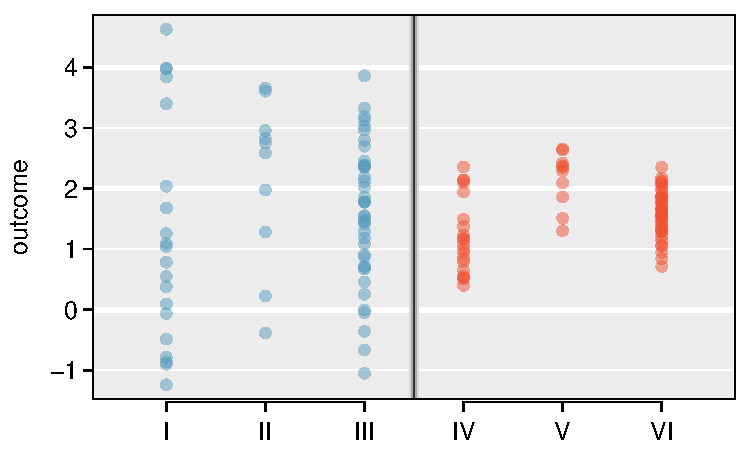
\includegraphics[width=0.75\textwidth]{08/figures/toyANOVA/toyANOVA}
\caption{Side-by-side dot plot for the outcomes for six groups.}
\label{toyANOVA}
\end{figure}
Any real difference in the means of groups I, II, and III is difficult to discern, because the data within each group are very volatile relative to any differences in the average outcome. On the other hand, it appears there are differences in the centers of groups IV, V, and VI. For instance, group IV appears to have a lower mean than that of the other two groups. Investigating groups IV, V, and VI, we see the differences in the groups' centers are noticeable because those differences are large \emph{relative to the variability in the individual observations within each group}.
\end{example}

\subsection{Is batting performance related to player position in MLB?}

We would like to discern whether there are real differences between the batting performance of baseball players according to their position: outfielder (\resp{OF}), infielder (\resp{IF}), designated hitter (\resp{DH}), and catcher (\resp{C}). We will use a data set called \data{mlbBat10}, which includes batting records of 327 Major League Baseball (MLB) players from the 2010 season. Six of the 327 cases represented in \data{mlbBat10} are shown in Table~\ref{mlbBat10DataMatrix}, and descriptions for each variable are provided in Table~\ref{mlbBat10Variables}. The measure we will use for the player batting performance (the outcome variable) is on-base percentage (\var{OBP}). The on-base percentage roughly represents the fraction of the time a player successfully gets on base or hits a home run.

\begin{table}[h]
\centering
\begin{tabular}{rlllrrrrrr}
  \hline
 & name & team & position & AB & H & HR &RBI & AVG & OBP \\ 
  \hline
1 & I Suzuki & SEA & OF & 680 & 214 & 6 & 43 & 0.315 & 0.359 \\ 
  2 & D Jeter & NYY & IF & 663 & 179 & 10 & 67 & 0.270 & 0.340 \\ 
  3 & M Young & TEX & IF & 656 & 186 & 21 & 91 & 0.284 & 0.330 \\ 
  $\vdots$ & $\vdots$ & $\vdots$ & $\vdots$ & $\vdots$ & $\vdots$ & $\vdots$ & $\vdots$ \\
  325 & B Molina & SF & C & 202 & 52 & 3 & 17 & 0.257 & 0.312 \\ 
  326 & J Thole & NYM & C & 202 & 56 & 3 & 17 & 0.277 & 0.357 \\ 
  327 & C Heisey & CIN & OF & 201 & 51 & 8 & 21 & 0.254 & 0.324 \\ 
   \hline
\end{tabular}
\caption{Six cases from the \data{mlbBat10} data matrix.}
\label{mlbBat10DataMatrix}
\end{table}

\begin{table}
\centering\small
\begin{tabular}{lp{9.5cm}}
\hline
{\bf variable} & {\bf description} \\
\hline
%\begin{itemize}
\var{name} & Player name \\
\var{team} & The player's team, where the team names are abbreviated \\
\var{position} & The player's primary field position (\resp{OF}, \resp{IF}, \resp{DH}, \resp{C}) \\
\var{AB} & Number of opportunities at bat \\
\var{H} & Number of hits \\
\var{HR} & Number of home runs \\
\var{RBI} & Number of runs batted in \\
\var{batAverage} & Batting average, which is equal to $\resp{H}/\resp{AB}$ \\
\hline
\end{tabular}
\caption{Variables and their descriptions for the \data{mlbBat10} data set.}
\label{mlbBat10Variables}
\end{table}

\begin{exercise} \label{nullHypForOBPAgainstPosition}
The null hypothesis under consideration is the following: $\mu_{\resp{OF}} = \mu_{\resp{IF}} = \mu_{\resp{DH}} = \mu_{\resp{C}}$.
Write the null and corresponding alternative hypotheses in plain language. Answers in the footnote\footnote{$H_0$: The average on-base percentage is equal across the four positions. $H_A$: The average on-base percentage varies across some (or all) groups.}.
\end{exercise}

%ZZQ Formatting
\pagebreak

\begin{example}{The player positions have been divided into four groups: outfield (\resp{OF}), infield (\resp{IF}), designated hitter (\resp{DH}), and catcher (\resp{C}). What would be an appropriate point estimate of the batting average by outfielders, $\mu_{\resp{OF}}$?}
A good estimate of the batting average by outfielders would be the sample average of \var{batAverage} for just those players whose position is outfield: $\bar{y}_{OF} = 0.334$.
\end{example}

Table~\ref{mlbHRPerABSummaryTable} provides summary statistics for each group. A side-by-side box plot for the batting average is shown in Figure~\ref{mlbANOVABoxPlot}. Notice that the variability appears to be approximately constant across groups; nearly constant variance across groups is an important assumption that must be satisfied before we consider the ANOVA approach.
\begin{table}[ht]
\centering\small
\begin{tabular}{lrrrr}
\hline
	& \resp{OF} & \resp{IF} & \resp{DH} & \resp{C} \\
\hline
Sample size ($n_i$)	& 120 & 154 & 14 & 39 \\
Sample mean ($\bar{y}_i$)	& 0.334 & 0.332 & 0.348 & 0.323 \\
Sample SD ($s_i$)	& 0.029 & 0.037 & 0.036 & 0.045 \\
\hline
\end{tabular}
\caption{Summary statistics of on-base percentage, split by player position.}
\label{mlbHRPerABSummaryTable}
\end{table}
\begin{figure}
\centering
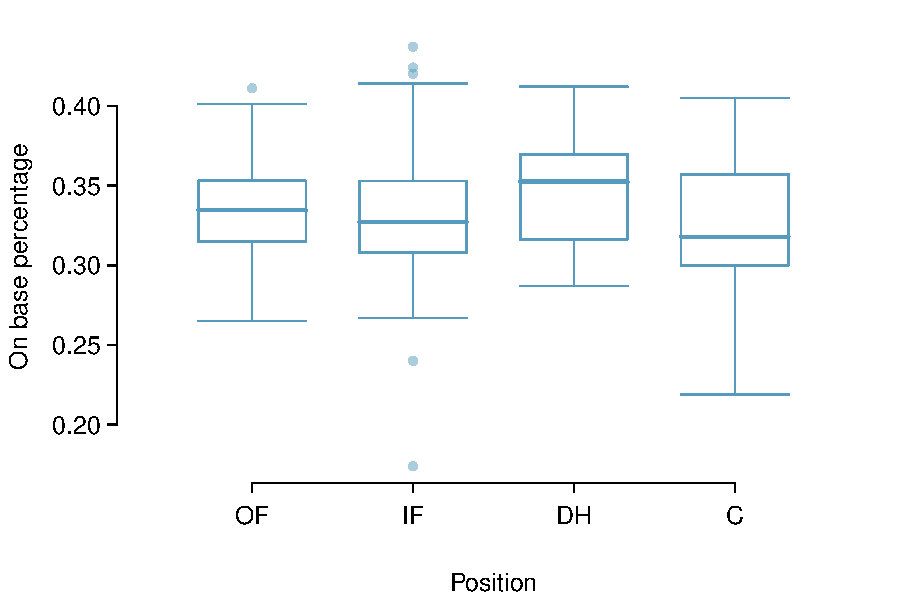
\includegraphics[width=0.85\textwidth]{08/figures/mlbANOVA/mlbANOVABoxPlot}
\caption{Side-by-side box plot of the on-base percentage for 327 players across four groups.}
\label{mlbANOVABoxPlot}
\end{figure}

\begin{example}{The largest difference between the sample means is between the designated hitter and the catcher positions. Consider again the original hypotheses:
\begin{itemize}
\setlength{\itemsep}{0mm}
\item[$H_0$:] $\mu_{\resp{OF}} = \mu_{\resp{IF}} = \mu_{\resp{DH}} = \mu_{\resp{C}}$
\item[$H_A$:] The average on-base percentage ($\mu_i$) varies across some (or all) groups.
\end{itemize}
Why might it be inappropriate to run the test by simply estimating whether the difference of $\mu_{\var{DH}}$ and $\mu_{\resp{C}}$ is statistically significant at a 0.05 significance level?}
\label{multipleComparisonExampleThatIncludesDiscussionOfClassrooms}
The primary issue here is that we are inspecting the data before picking the groups that will be compared. It is inappropriate to examine all data by eye (informal testing) and only afterwards decide which parts to formally test. This is called \term{data snooping} or \term{data fishing}. Naturally we would pick the groups with the large differences for the formal test, leading to an unintentional inflation in the Type 1 Error rate. To understand this better, let's consider a slightly different problem.

Suppose we are to measure the aptitude for students in 20 classes in a large elementary school at the beginning of the year. In this school, all students are randomly assigned to classrooms, so any differences we observe between the classes at the start of the year are completely due to chance. However, with so many groups, we will probably observe a few groups that look rather different from each other. If we select only these classes that look so different, we will probably make the wrong conclusion that the assignment wasn't random. While we might only formally test differences for a few pairs of classes, we informally evaluated the other classes by eye before choosing the most extreme cases for a comparison.
\end{example}

For additional reading on the ideas expressed in Example~\ref{multipleComparisonExampleThatIncludesDiscussionOfClassrooms}, we recommend reading about the \term{prosecutor's fallacy}\footnote{See, for example, \url{http://www.stat.columbia.edu/~cook/movabletype/archives/2007/05/the_prosecutors.html}.}.

In the next section we will learn how to use the $F$ statistic and ANOVA to test whether differences in means could have happened just by chance.

\subsection{Analysis of variance (ANOVA) and the $F$ test}

The method of analysis of variance focuses on answering one question: is the variability in the sample means so large that it seems unlikely to be from chance alone? This question is different from earlier testing procedures since we will \emph{simultaneously} consider many groups, and evaluate whether their sample means differ more than we would expect from natural variation. We call this variability the \term{mean square between groups ($MSG$)}, and it has an associated degrees of freedom, $df_{G}=k-1$ when there are $k$ groups. The $MSG$ is sort of a scaled variance formula for means. If the null hypothesis is true, any variation in the sample means is due to chance and shouldn't be too large%; it should be roughly equal to the variability in the outcome variable
. Details of $MSG$ calculations are provided in the footnote\footnote{Let $\bar{y}$ represent the mean of outcomes across all groups. Then the mean square between groups is computed as
\begin{align*}
MSG = \frac{1}{df_{G}}SSG = \frac{1}{k-1}\sum_{i=1}^{k} n_{i}\left(\bar{y}_{i} - \bar{y}\right)^2
\end{align*}
where $SSG$ is called the \term{sum of squares between groups} and $n_{i}$ is the sample size of group $i$.}, however, we typically use software for these computations.

The mean square between the groups is, on its own, quite useless in a hypothesis test. We need a benchmark value for how much variability should be expected among the sample means if the null hypothesis is true. To this end, we compute the mean of the squared errors, often abbreviated as the \term{mean square error ($MSE$)}, which has an associated degrees of freedom value $df_E=n-k$. It is helpful to think of $MSE$ as a measure of the variability of the residuals. Details of the computations of the $MSE$ are provided in the footnote\footnote{Let $\bar{y}$ represent the mean of outcomes across all groups. Then the \term{sum of squares total ($SST$)} is computed as
\begin{align*}
SST = \sum_{i=1}^{n} \left(y_{i} - \bar{y}\right)^2
\end{align*}
where the sum is over all observations in the data set. Then we compute the \term{sum of squared errors ($SSE$)} in one of three equivalent ways:
\begin{align*}
SSE &= SST - SSG \\
	&= (n_1-1)*s_1^2 + (n_2-1)*s_2^2 + \cdots + (n_k-1)*s_k^2 \\
	&= \sum_{j=1}^{n} e_i^2
\end{align*}
where $s_i^2$ is the sample variance (square of the standard deviation) of the residuals in group $i$, and the last expression represents the sum of the squared residuals across all groups. Then the $MSE$ is the standardized form of $SSE$: $MSE = \frac{1}{df_{E}}SSE$.} for the interested reader.

When the null hypothesis is true, any differences among the sample means are only due to chance, and the $MSG$ and $MSE$ should be about equal. As a test statistic for ANOVA, we examine the fraction of $MSG$ and $MSE$:
\begin{align} \label{formulaForTheFStatistic}
F = \frac{MSG}{MSE}
\end{align}
The $MSG$ represents a measure of the between-group variability, and $MSE$ the variability within each of the groups.

\begin{exercise}
For the baseball data, $MSG = 0.00252$ and $MSE=0.00127$. Identify the degrees of freedom associated with each mean square and verify the $F$ statistic is 1.994.
\end{exercise}

We use the $F$ statistic to evaluate the hypotheses in what is called an \term{F test}. We compute a p-value from the $F$ statistic using an $F$ distribution, which has two associated parameters: $df_{1}$ and $df_{2}$. For the $F$ statistic in ANOVA, $df_{1} = df_{G}$ and $df_{2}= df_{E}$. An $F$ distribution with 3 and 323 degrees of freedom, corresponding to the $F$ statistic for the baseball hypothesis test, is shown in Figure~\ref{fDist3And323}.
\begin{figure}[ht]
\centering
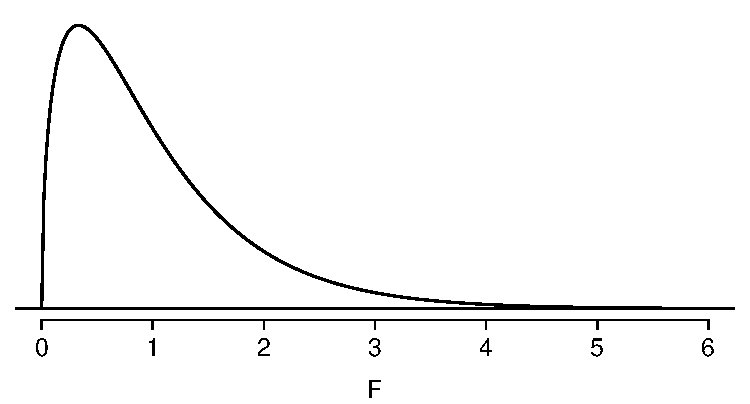
\includegraphics[width=0.7\textwidth]{08/figures/fDist3And323/fDist3And323}
\caption{An $F$ distribution with $df_1=3$ and $df_2=323$.}
\label{fDist3And323}
\end{figure}

The larger the observed variability in the sample means ($MSG$) relative to the residuals ($MSE$), the larger $F$ will be and the stronger the evidence against the null hypothesis. Because larger values of $F$ represent stronger evidence against the null hypothesis, we use the upper tail of the distribution to compute a p-value.

\begin{termBox}{\tBoxTitle{The $F$ statistic and the $F$ test}
Analysis of variance (ANOVA) is used to test whether the mean outcome differs across 2 or more groups. ANOVA uses a test statistic $F$, which represents a standardized ratio of variability in the sample means relative to the variability of the residuals. If $H_0$ is true and the model assumptions are satisfied, the statistic $F$ follows an $F$ distribution with parameters $df_{1}=k-1$ and $df_{2}=n-k$. The upper tail of the $F$ distribution is used to represent the p-value.}
\end{termBox}

\begin{exercise}\label{describePValueAreaForFDistributionInMLBOBPExample}
The test statistic for the baseball example is $F=1.994$. Shade the area corresponding to the p-value in Figure~\ref{fDist3And323}.
\end{exercise}

\begin{example}{The p-value corresponding to the solution for Exercise~\ref{describePValueAreaForFDistributionInMLBOBPExample} is equal to about 0.115. Does this provide strong evidence against the null hypothesis?}
The p-value is larger than 0.05, indicating the evidence is not sufficiently strong to reject the null hypothesis at a significance level of 0.05. That is, the data do not provide strong evidence that the average on-base percentage varies by player's primary field position.
\end{example}

\subsection{Reading regression and ANOVA output from software}

The calculations required to perform an ANOVA by hand are tedious and prone to human error. For these reasons it is common to use a statistical software to calculate the $F$ statistic and p-value.

An ANOVA can be summarized in a table very similar to that of a regression summary. Table~\ref{anovaSummaryTableForOBPAgainstPosition} shows an ANOVA summary to test whether the mean of on-base percentage varies by player positions in the MLB.
\begin{table}[ht]
\centering
\begin{tabular}{lrrrrr}
  \hline
 & Df & Sum Sq & Mean Sq & F value & Pr($>$F) \\ 
  \hline
position & 3 & 0.0076 & 0.0025 & 1.9943 & 0.1147 \\ 
  Residuals & 323 & 0.4080 & 0.0013 &  &  \\    \hline
\multicolumn{6}{r}{$s_{pooled} = 0.036$ on $df=323$}
\end{tabular}
\caption{ANOVA summary for testing whether the average on-base percentage differs across player positions.}
\label{anovaSummaryTableForOBPAgainstPosition}
\end{table}

\begin{exercise}
Earlier you verified that the $F$ statistic for this analysis was 1.994, and the p-value of 0.115 was provided. Circle these values in Table~\ref{anovaSummaryTableForOBPAgainstPosition} and notice the corresponding column name. Notice that both of these values are in the row labeled \emph{position}, which corresponds to the categorical variable representing the player position variable.
\end{exercise}

\begin{exercise}
The $s_{pooled}=0.036$ on $df=323$ describes the estimated standard deviation associated with the residuals. Verify that $s_{pooled}$ equals the square root of the $MSE$ for the \emph{Residuals} row.
\end{exercise}

\subsection{Graphical diagnostics for an ANOVA analysis}

There are three primary conditions we must check for an ANOVA analysis, all related to the residuals (errors) associated with the model. Recall that we assume the errors are independent, nearly normal, and have nearly constant variance across the groups.

\begin{description}
\item[Independence.] If observations are collected in a particular order, we should plot the residuals in the order the corresponding observations were collected (e.g. see Figure~\ref{mkDiagnosticInOrder} on page~\pageref{mkDiagnosticInOrder}). For the baseball data, the data were collected from a sorted table, making such a review impossible. However, we can consider the nature of the data: Do we have reason to believe players are not independent? There are not obvious reasons why independence should not hold, so we will assume independence is reasonable in lieu of being able to examine this condition using data.
\item[Approximately normal.] The normality assumption for the residuals is especially important when the sample size is quite small. Figure~\ref{mlbANOVADiagNormality} shows a normal probability plot for the residuals from the baseball data. We do see some deviation from normality at the low end, where there is a longer tail than what we would expect if the residuals were truly normal. While we should report this finding with the results of the hypothesis test, this slight deviation probably has little impact on the test results since there are so many players included in the sample and they are not spread thinly across many groups. % but can be slightly relaxed for residuals of groups with larger sample sizes. We do see some deviations from normality in the lower tail. However, the three smallest residuals are from the infield and outfield groups. Because each of these groups each contain over 100 cases, so the potential outliers probably alright (but these observations are worth mentioning in a report of the analysis).
\begin{figure}
\centering
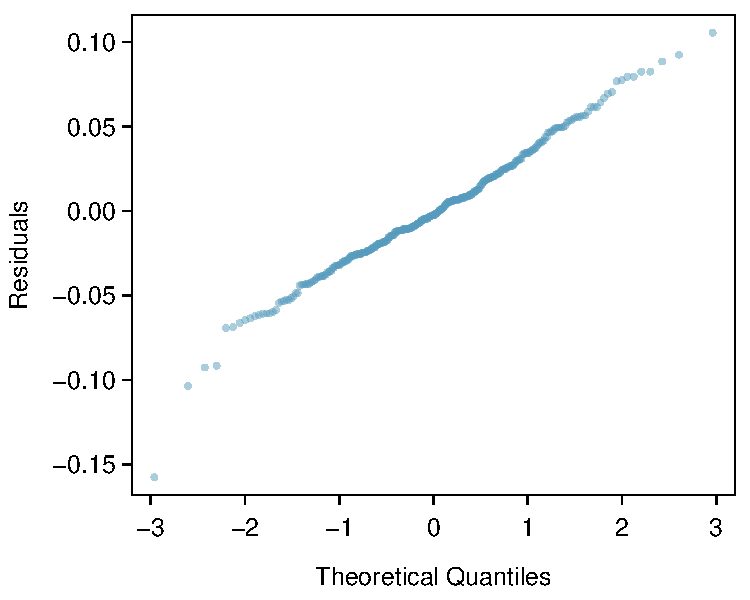
\includegraphics[width=0.75\textwidth]{08/figures/mlbANOVA/mlbANOVADiagNormality}
\caption{Normal probability plot of the residuals.}
\label{mlbANOVADiagNormality}
\end{figure}
\item[Constant variance.] The last assumption is that the variance associated with the residuals is nearly constant from one group to the next. This assumption can be checked by examining a side-by-side box plot of the outcomes, as in Figure~\ref{mlbANOVABoxPlot}. In this case, the variability is similar in the four groups but not identical. We see in Table~\ref{mlbHRPerABSummaryTable} on page~\pageref{mlbHRPerABSummaryTable} that the standard deviation varies a bit from one group to the next. Whether these differences are from natural variation is unclear, so we should report this uncertainty with the final results.
%\begin{figure}
%\centering
%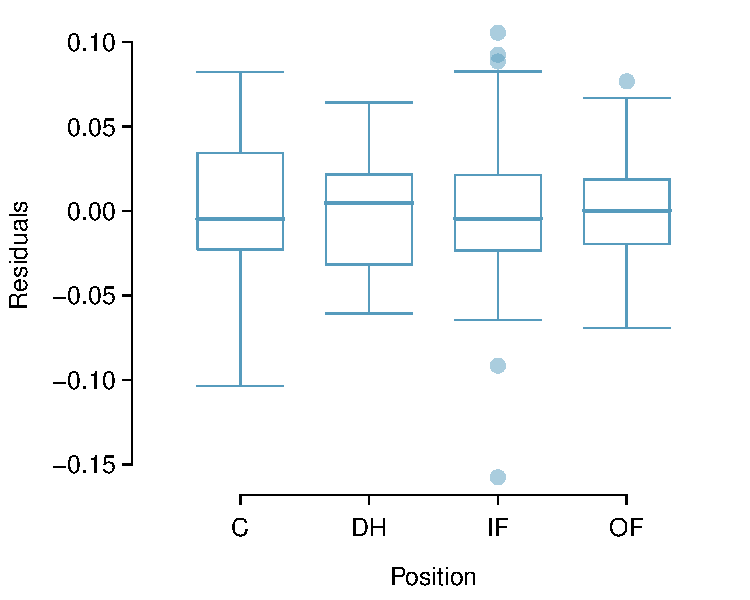
\includegraphics[width=0.75\textwidth]{08/figures/mlbANOVA/mlbANOVADiagConstantVar}
%\caption{Side-by-side box plot of the residuals in their corresponding groups.}
%\label{mlbANOVADiagConstantVar}
%\end{figure}
\end{description}

\begin{caution}
{Diagnostics for an ANOVA analysis}
{Independence is always important to an ANOVA analysis. The normality condition is very important when the sample sizes for each group are relatively small. The constant variance condition is especially important when the sample sizes differ between groups.}
\end{caution}

\subsection{Multiple comparisons and controlling Type 1 Error rate}
\label{multipleComparisonsAndControllingTheType1ErrorRate}

When we reject the null hypothesis in an ANOVA analysis, we might wonder, which of these groups have different means? To answer this question, we compare the means of each possible pair of groups. For instance, if there are three groups and there is strong evidence that there are some differences in the group means, there are three comparisons to make: group 1 to group 2, group 1 to group 3, and group 2 to group 3. These comparisons can be accomplished using a two-sample $t$ test, but we must use a modified significance level and a pooled estimate of the standard deviation across groups.

\begin{example}{Example~\ref{firstExampleForThreeStatisticsClassesAndANOVA} on page~\pageref{firstExampleForThreeStatisticsClassesAndANOVA} discussed three statistics lectures, all taught during the same semester. Table~\ref{summaryStatisticsForClassTestData} shows summary statistics for these three courses, and a side-by-side box plot of the data is shown in Figure~\ref{classDataSBSBoxPlot}. We would like to conduct an ANOVA for these data. Do you see any deviations from the three conditions for ANOVA?}
In this case (like many others) it is difficult to check independence in a rigorous way. Instead, the best we can do is use common sense to consider reasons the assumption of independence may not hold. For instance, the independence assumption may not be reasonable if there is a star teaching assistant that only half of the students may access; such a scenario would divide a class into two subgroups. After carefully considering the data, we believe that assuming independence may be acceptable.

The distributions in the side-by-side box plot appear to be roughly symmetric and show no noticeable outliers.

The box plots show approximately equal variability, which can be verified in Table~\ref{summaryStatisticsForClassTestData}, supporting the constant variance assumption.
\end{example}
\begin{table}[ht]
\centering
\begin{tabular}{lrrr}
  \hline
Class $i$	& A	& B	& C \\ 
  \hline
$n_i$		& 58	& 55	& 51 \\ 
$\bar{y}_i$	& 75.1	& 72.0	& 78.9 \\ 
$s_i$		& 13.9	& 13.8	& 13.1 \\ 
\hline
\end{tabular}
\caption{Summary statistics for the first midterm scores in three different lectures of the same course.}
\label{summaryStatisticsForClassTestData}
\end{table}
\begin{figure}[ht]
\centering
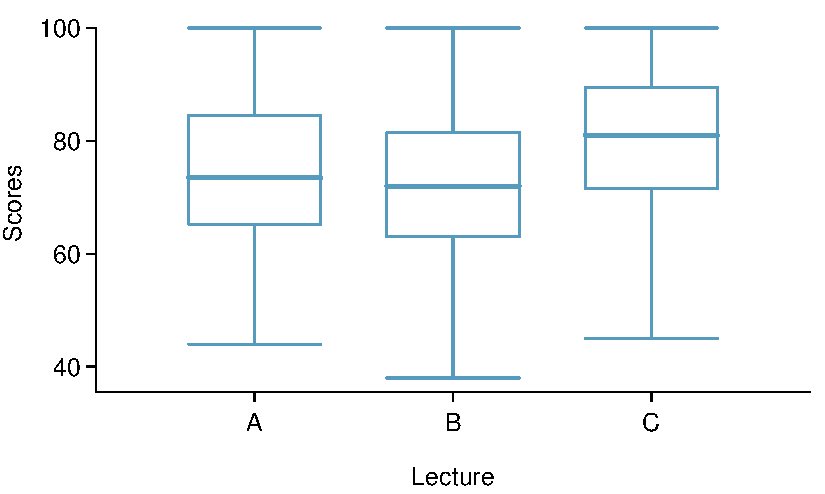
\includegraphics[width=0.8\textwidth]{08/figures/classData/classDataSBSBoxPlot}
\caption{Side-by-side box plot for the first midterm scores in three different  lectures of the same course.}
\label{classDataSBSBoxPlot}
\end{figure}

\begin{exercise} \label{exerExaminingAnovaSummaryTableForMidtermData}
An ANOVA was conducted for the midterm data, and a summary is shown in Table~\ref{anovaSummaryTableForMidtermData}. What should we conclude?
\end{exercise}

\begin{table}[ht]
\centering
\begin{tabular}{lrrrrr}
  \hline
 & Df & Sum Sq & Mean Sq & F value & Pr($>$F) \\ 
  \hline
lecture & 2 & 1290.11 & 645.06 & 3.48 & 0.0330 \\ 
  Residuals & 161 & 29810.13 & 185.16 &  &  \\ 
   \hline
\multicolumn{6}{r}{$s_{pooled}=13.61$ on $df=161$}
\end{tabular}
\caption{ANOVA summary table for the midterm data.}
\label{anovaSummaryTableForMidtermData}
\end{table}

%\Comment{Need to include SD estimate from analysis in tables AND use it in multiple comparisons below.}

There is strong evidence that the different means in each of the three classes is not simply due to chance. We might wonder, which of the classes are actually different? As discussed in earlier chapters, a two-sample $t$ test could be used to test for differences in each possible pair of groups. However, one pitfall was discussed in Example~\ref{multipleComparisonExampleThatIncludesDiscussionOfClassrooms} on page~\pageref{multipleComparisonExampleThatIncludesDiscussionOfClassrooms}: when we run so many tests, the Type~1 Error rate increases. This issue is resolved by using a modified significance level.

\begin{termBox}{\tBoxTitle{Multiple comparisons and the Bonferroni correction for $\alpha$}
The scenario of testing many pairs of groups is called \term{multiple comparisons}. The \term{Bonferroni correction} suggests that a more stringent significance level is more appropriate for these tests:
\begin{align*}
\alpha^* = \alpha / K
\end{align*}
where $K$ is the number of comparisons being considered (formally or informally). If there are $k$ groups, then usually all possible pairs are compared and $K=\frac{k(k-1)}{2}$.}
\end{termBox}

\begin{example}{In Exercise~\ref{exerExaminingAnovaSummaryTableForMidtermData}, you found that the data showed strong evidence of differences in the average midterm grades between the three lectures. Complete the three possible pairwise comparisons using the Bonferroni correction and report any differences.} \label{multipleComparisonsOfThreeStatClasses}
We use a modified significance level of $\alpha^* = 0.05/3 = 0.0167$. Additionally, we use the pooled estimate of the standard deviation: $s_{pooled}=13.61$ on $df=161$.

Lecture A versus Lecture B: The estimated difference and standard error are, respectively,
\begin{align*}
\bar{y}_A - \bar{y}_{B} &= 75.1 - 72 = 3.1
	&SE = \sqrt{\frac{13.61^2}{58} + \frac{13.61^2}{55}} &= 2.56
\end{align*}
(See Section~\ref{pooledStandardDeviations} on page~\ref{pooledStandardDeviations} for additional details.) This results in a $T$ score of 1.21 on $df = 161$ (we use the $df$ associated with $s_{pooled}$) and a two-tailed p-value of 0.228. This p-value is larger than $\alpha^*=0.0167$, so there is not strong evidence of a difference in the means of lectures A and B.

Lecture A versus Lecture C: The estimated difference and standard error are 3.8 and 2.61, respectively. This results in a $T$ score of 1.46 on $df = 161$ and a two-tailed p-value of 0.1462. This p-value is larger than $\alpha^*$, so there is not strong evidence of a difference in the means of lectures A and C.

Lecture B versus Lecture C: The estimated difference and standard error are 6.9 and 2.65, respectively. This results in a $T$ score of 2.60 on $df = 161$ and a two-tailed p-value of 0.0102. This p-value is smaller than $\alpha^*$. Here we find strong evidence of a difference in the means of lectures B and C.
\end{example}

We might summarize the findings of the analysis from Example~\ref{multipleComparisonsOfThreeStatClasses} using the following notation:
\begin{align*}
\mu_A &\stackrel{?}{=} \mu_B
	&\mu_A &\stackrel{?}{=} \mu_C
	&\mu_B &\neq \mu_C
\end{align*}
The midterm mean in lecture A is not statistically distinguishable from those of lectures B or C. However, there is strong evidence that lectures B and C are different. In the first two pairwise comparisons, we did not have sufficient evidence to reject the null hypothesis. Recall that failing to reject $H_0$ does not imply $H_0$ is true.

\begin{caution}
{Sometimes an ANOVA will reject the null but no groups will have statistically significant differences}
{It is possible to reject the null hypothesis using ANOVA and then to not subsequently identify differences in the pairwise comparisons. However, \emph{this does not invalidate the ANOVA conclusion}. It only means we have not been able to successfully identify which groups differ in their means.}
\end{caution}

The ANOVA procedure examines the big picture: it considers all groups simultaneously to decipher whether there is evidence that some difference exists. Even if the test indicates that there is strong evidence of differences in group means, identifying with high confidence a specific difference as statistically significant is more difficult.

Consider the following analogy: we observe a Wall Street firm that makes large quantities of money based on predicting mergers. Mergers are generally difficult to predict, and if the prediction success rate is extremely high, that may be considered sufficiently strong evidence to warrant investigation by the Securities and Exchange Commission (SEC). While the SEC may be quite certain that there is insider trading taking place at the firm, the evidence against any single trader may not be very strong. It is only when the SEC considers all the data that they identify the pattern. This is effectively the strategy of ANOVA: stand back and consider all the groups simultaneously.

\subsection{Using ANOVA for multiple regression}

The ANOVA methodology can be extended to multiple regression, where we simultaneously incorporate categorical and numerical predictors into a model. The methods discussed so far -- an outcome for a single categorical variable -- is called \term{one-way ANOVA}. There are two extensions that we briefly discuss here: evaluating all variables in a model simultaneously, and using ANOVA in model selection where some variables are numerical and others categorical.

Some software will supply additional information about a multiple regression model fit beyond the regression summaries described in this textbook. This additional information can be used in an assessment of the utility of the full model. For instance, below is the full regression summary for the Mario Kart Wii game analysis from Section~\ref{modelSelection} (implemented with R statistical software\footnote{R is free and can be downloaded at \url{www.r-project.org}.}) using all four predictors:
\begin{verbatim}
    Residuals:
         Min       1Q   Median       3Q      Max 
    -11.3788  -2.9854  -0.9654   2.6915  14.0346 
    
    Coefficients:
                Estimate Std. Error t value Pr(>|t|)    
    (Intercept) 36.21097    1.51401  23.917  < 2e-16 ***
    condNew      5.13056    1.05112   4.881 2.91e-06 ***
    stockPhoto   1.08031    1.05682   1.022    0.308    
    duration    -0.02681    0.19041  -0.141    0.888    
    wheels       7.28518    0.55469  13.134  < 2e-16 ***
    ---
    Signif. codes:  0 �***� 0.001 �**� 0.01 �*� 0.05 �.� 0.1 � � 1 
    
    Residual standard error: 4.901 on 136 degrees of freedom
    Multiple R-squared: 0.719,	Adjusted R-squared: 0.7108 
    F-statistic: 87.01 on 4 and 136 DF,  p-value: < 2.2e-16 
\end{verbatim}
The main output labeled \texttt{Coefficients} should be familiar as the multiple regression summary. The last three lines are new and provide details about
\begin{itemize}
\setlength{\itemsep}{0mm}
\item the standard deviation associated with the residuals (4.901),
\item degrees of freedom (136),
\item $R^2$ (0.719) and adjusted $R^2$ (0.7108), and
\item also an $F$ statistic (174.4 with $df_1=4$ and $df_2=136$) with an associated p-value ($<$2.2e-16, i.e. about zero).
\end{itemize}
The $F$ statistic and p-value in the last line can be used for a test of the entire model. The p-value can be used to the answer the following question: Is there strong evidence that the model as a whole is significantly better than using no variables? In this case, with a p-value of less than $2.2\times10^{-16}$, there is extremely strong evidence that the variables included are helpful in prediction. Notice that the p-value does not verify that all variables are actually important in the model; it only considers the importance of all of of the variables simultaneously. This is similar to how ANOVA was earlier used to assess differences across all means without saying anything about the difference between a particular pair of means.

The second setting for ANOVA in the general multiple regression framework is one that is more delicate: model selection. We could compare the variability in the residuals of two models that differ by just one predictor using ANOVA as a tool to evaluate whether the data support the inclusion of that variable in the model. We postpone further details of this method to a later course.

%\begin{caution}
%{Read software carefully before applying ANOVA to variable selection in multiple regression}
%{The way ANOVA is applied in a multiple regression for model selection is complex. Do not apply ANOVA in a model selection framework without first understanding how to obtain proper p-values for predictor variables.}
%\end{caution}

%\Summary{Connect salary data to the }


%%%%%
%\section{Logistic regression for a binomial outcome}

%\subsection{Evaluating the 2010 House election using 2008 results}

%\subsection{Modeling the probability of an event}

%\subsection{Fitting a model to}




